%% LyX 2.3.7 created this file.  For more info, see http://www.lyx.org/.
%% Do not edit unless you really know what you are doing.
\documentclass[spanish]{article}
\usepackage[T1]{fontenc}
\usepackage{amssymb}
\usepackage[final]{graphicx}

\makeatletter
%%%%%%%%%%%%%%%%%%%%%%%%%%%%%% User specified LaTeX commands.
\usepackage{palatino}

\makeatother

\usepackage{babel}
\addto\shorthandsspanish{\spanishdeactivate{~<>}}

\begin{document}
\title{Trabajo pr\'{a}ctico 1: Bayes Ingenuo}
\author{Ph. D. Sa\'{u}l Calder\'{o}n Ram\'{\i}rez \\
Instituto Tecnol\'{o}gico de Costa Rica, \\
Escuela de Ingenier\'{\i}a en Computaci\'{o}n, Programa de Ciencias
de Datos,\\
PAttern Recongition and MAchine Learning Group (PARMA-Group)}

\maketitle
\textbf{Fecha de entrega:} Domingo 12 de Mayo

\textbf{Entrega}: Un archivo .zip con el c\'{o}digo fuente LaTeX o
Lyx, el pdf, y un notebook Jupyter, debidamente documentado, con una
funci\'{o}n definida por ejercicio. A trav\'{e}s del TEC-digital.

\textbf{Modo de trabajo}: Grupos de 3 personas.
\begin{abstract}
En el presente trabajo pr\'{a}ctico se introduce la implementaci\'{o}n
de redes bayesianas. El trabajo practico consta de 120 puntos, donde
20 son extra.
\end{abstract}

\section{(40 puntos) Implementaci\'{o}n de la clasificaci\'{o}n multi-clase
de im\'{a}genes con Bayes ingenuo usando histogramas}

\begin{enumerate}
    \item Para el presente ejercicio, se implementar\'{a} la clasificaci\'{o}n
    de imagenes naturales con $K=10$ clases. La Figura \ref{fig:Imagenes-de-CIFAR-10.}
    muestra algunas observaciones del conjunto de datos. El c\'{o}digo
    provisto lee las im\'{a}genes del conjunto de datos, y los transforma
    a matrices binarias de $32\times32=1024$ pixeles. El objetivo de
    su equipo de desarrollo es utilizar el teorema de Bayes para construir
    un modelo conocido como Bayes ingenuo, el cual permita estimar la
    clase a la que pertenece una nueva observaci\'{o}n.

    \begin{figure}
        \begin{centering}
        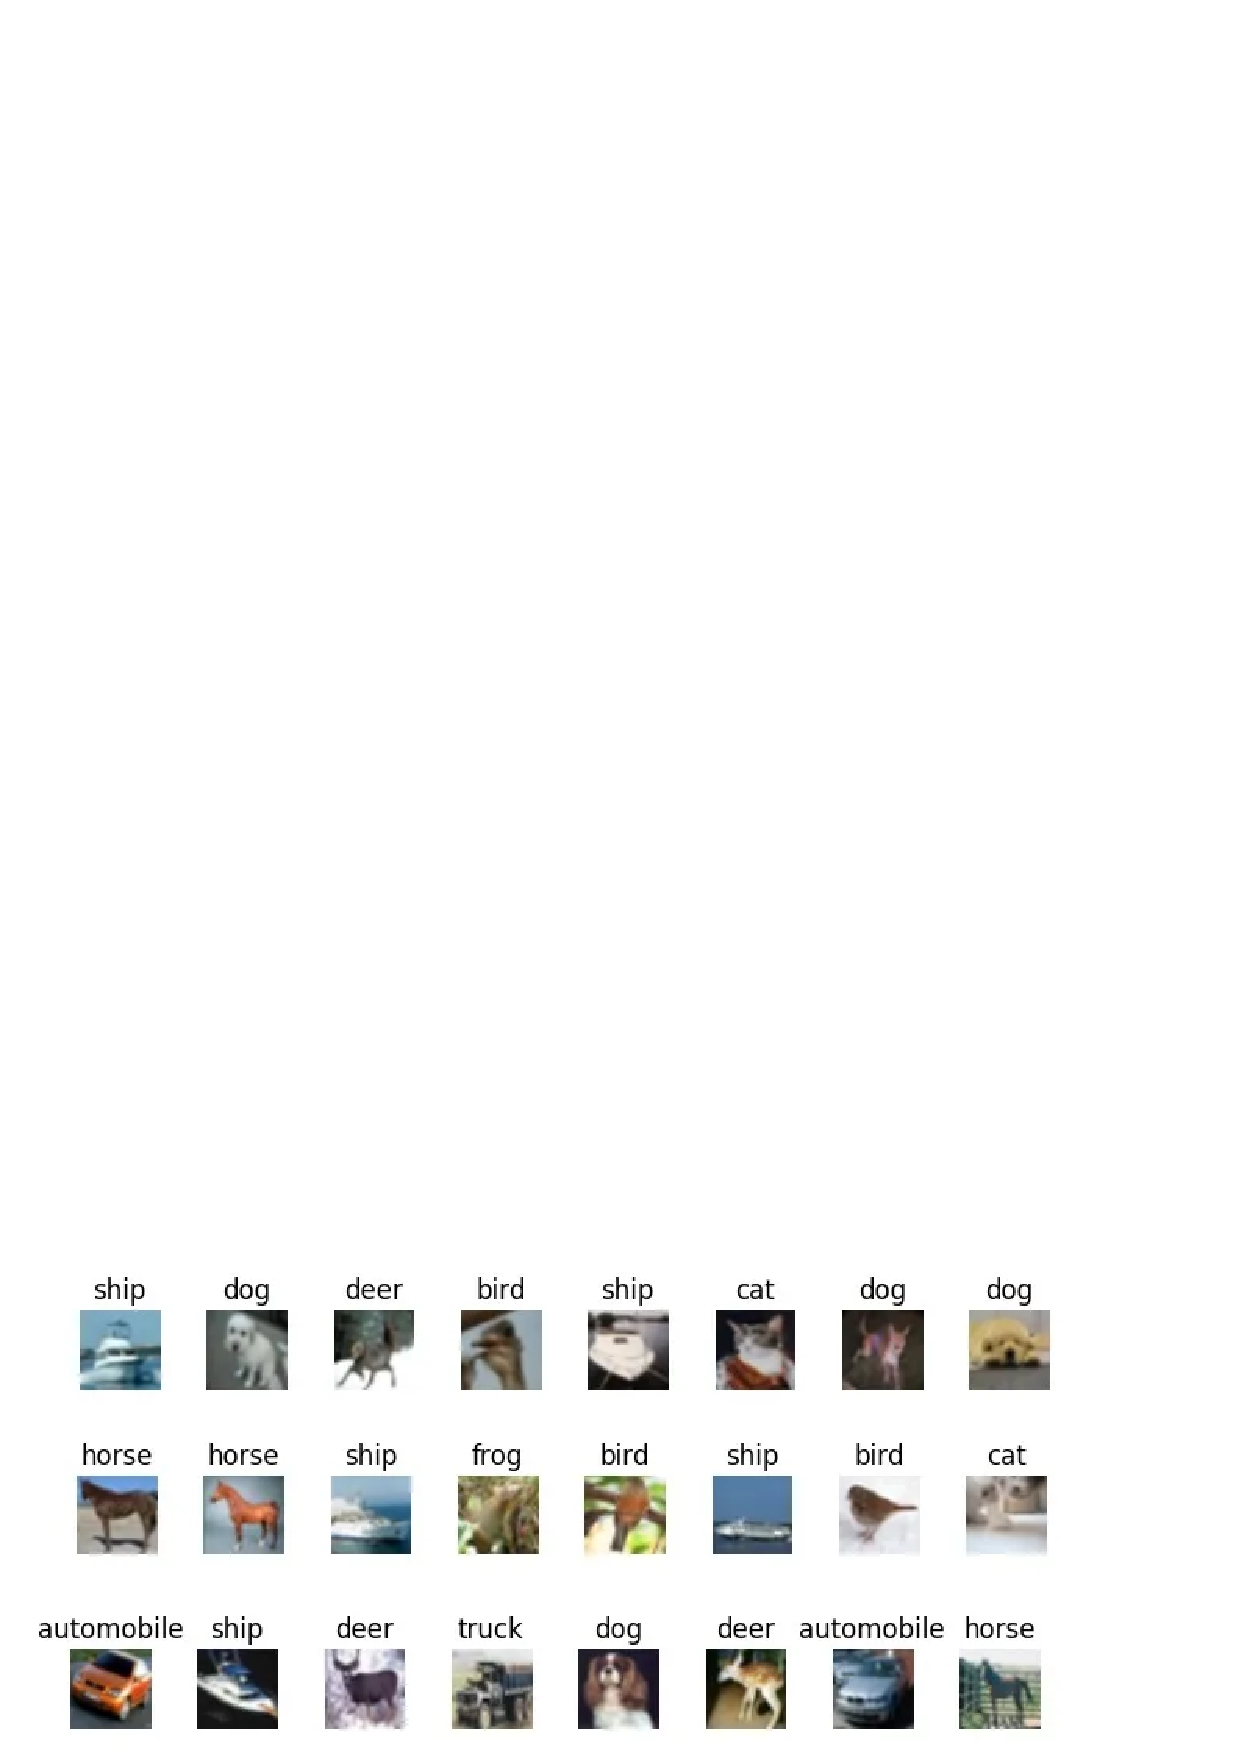
\includegraphics[scale=0.7]{TP1_Bayes/Images/cifar10.png}
        \par
        \end{centering}
        \caption{Imagenes de CIFAR-10.
        \label{fig:Imagenes-de-CIFAR-10.}}
    \end{figure}

    \item En el material del curso, se discute el algoritmo de Bayes ingenuo,
    el cual tiene por objetivo estimar la \textbf{probabilidad posterior}
    de que una observaci\'{o}n (imagen en este caso) $\overrightarrow{m}\in\mathbb{N}^{D},$donde
    en este caso $D=1024$, pertenezca a una clase $k$ como:
        \[
        \begin{array}{c}
        p\left(t=k|\overrightarrow{m}\right)\end{array}
        \]
        
    Para aproximarla, se utiliza el teorema de Bayes, el cual luego de
    desarrollar y simplificar la expresion de tal probabilidad posterior,
    se concluye que esta es proporcional a la multiplicaci\'{o}n de la
    probabilidad a priori de $p\left(t=k\right)$ y la verosimilitud de
    un pixel $p\left(m_{i}|t=k\right)$:
        \[
        p\left(t=k|\overrightarrow{m}\right)\propto\prod_{i=0}^{D}p\left(m_{i}|t=k\right)p\left(t=k\right).
        \]
        
    Por ejemplo, la verosimilitud del pixel $i$ negro (0), $p\left(m_{i}|t=k\right)$
    se implementa como la probablididad de que $p\left(m_{i}=0|t=k\right)$
    en caso de que ese pixel $i$ de la observaci\'{o}n a evaluar en el
    modelo sea negro (0). Es necesario calcular la verosimilitud de cada
    intensidad de pixel $p\left(m_{i}=0|t=k\right)$,
    $p\left(m_{i}=1|t=k\right)$,$p\left(m_{i}=2|t=k\right)$
    hasta $p\left(m_{i}=255|t=k\right)$ ($Z=255$).
    
    \begin{enumerate}
        \item \textbf{(10 puntos)} Implemente el c\'{a}lculo de las probabilidades
        a priori $p\left(t\right)$ para las $K=10$ clases en el conjunto
        de datos de entrenamiento en la funci\'{o}n \emph{calcular\_probabilidad\_priori}.
        Realice tal calculo dentro de la funcion \emph{train\_model. }
        
        \item Dise\~{n}e y muestre el resultado de una o m\'{a}s pruebas unitarias
        de tal funci\'{o}n objetivo, entradas, salidas esperadas y resultados). 
    \end{enumerate}

    \begin{enumerate}
        \item Para evaluar la verosimilitud $p\left(m_{d}|t\right)$, es necesario
        estimar las densidades $p\left(m_{d}=0|t\right)$,... $p\left(m_{d}=255|t\right),$
        para todos los pixeles $d=1,\ldots1024$ pixeles. Para ello, su equipo
        considerar\'{a} las siguientes dos variantes:
        \begin{enumerate}
            \item \textbf{Enfoque basado en histogramas}: Siguiendo la simplificaci\'{o}n
            sugerida por su colega Josef, usando las im\'{a}genes binarizadas,
            se sugiere lo siguiente. Cree un \textbf{tensor}\textbf{\emph{ }}\textbf{de
            dimensiones }\textbf{\emph{dataset\_densities}}\textbf{ }$D\times Z\times K$\emph{,
            }el cual represente las densidades de cada pixel (1024 en total) para
            cada una de las intensidades de pixel posibles ($Z=255$ maximo) para
            cada una de las clases ($K$ clases en total), por lo que entonces
            cada columna corresponde a la densidad de cada pixel. \textbf{Para
            realizar este calculo solo se le permite usar un ciclo }\textbf{\emph{for,
            }}\textbf{con una iteracion por clase $k$, como maximo}. Estime los
            valores de tal matriz usando el conjunto de datos de entrenamiento.
            
            \item \textbf{(20 puntos)} Implemente los dos puntos anteriores en la funci\'{o}n
            \emph{train\_model\_histogram }y retorne \emph{dataset\_densities},
            junto con el arreglo de probabilidades a priori para todas las clases. 

            \item Dise\~{n}e y muestre el resultado de dos o m\'{a}s pruebas unitarias
            de tal funci\'{o}n (objetivo, entradas, salidas esperadas y resultados).
            
            \item Grafique los histogramas de los primeros 5 pixeles y las primeras
            5 intensidades de pixeles para la clase 1 y 2. Siguen alguna distribucion
            conocida?
            
        \end{enumerate}
        
\item \textbf{(5 puntos)} Implemente la funci\'{o}n \emph{test\_model\_histogram(input\_torch,
dataset\_densities, num\_classes = 10) }la cual realice la estimaci\'{o}n
de a cual clase pertenece una observaci\'{o}n contenida en el vector
\emph{input\_torch, }para un modelo representado en \emph{dataset\_densities
(}obtenido en el paso anterior\emph{). }Para ello, el enfoque de Bayes
ingenuo estima la funci\'{o}n de densidad posterior como sigue:
\[
p\left(t=k|\overrightarrow{m}\right)\propto\prod_{d=0}^{D}p\left(m_{d}|t=k\right)p\left(t=k\right).
\]
La clase estimada a la que pertenece la observaci\'{o}n $\overrightarrow{m}$
corresponde entonces a la clase $k$ con mayor probabilidad posterior
$p\left(t=k|\overrightarrow{m}\right)$. 
\begin{enumerate}
\item Dise\~{n}e y muestre el resultado de una o m\'{a}s pruebas unitarias
de tal funci\'{o}n, siguiendo las pautas del dise\~{n}o anteriores.
Explique el dise\~{n}o de la misma. 
\end{enumerate}
\item \textbf{(5 puntos)} Implemente la funci\'{o}n \emph{test\_model\_batch\_histogram(test\_set,
labels, dataset\_densities, p\_t\_tensor) }la cual calcule y retorne
la tasa de aciertos para un conjunto de observaciones, basado en la
funci\'{o}n anteriormente implementada \emph{test\_model.}
\begin{enumerate}
\item Dise\~{n}e y muestre los resultados de al menos 2 pruebas unitarias
para validar su correcto funcionamiento. Detalle el dise\~{n}o y documente
los resultados obtenidos de las dos pruebas unitarias.
\end{enumerate}
\end{enumerate}
\end{enumerate}

\subsection{(30 puntos) Prueba del modelo}
\begin{enumerate}
\item \textbf{(10 puntos)} Entrene el modelo propuesto, con el conjunto
de observaciones contenido en la carpeta \emph{train}, y reporte la
tasa de aciertos al utilizar la funci\'{o}n anteriormente implementada\emph{test\_model\_batch\_histogram}.
Verifique y comente los resultados. Es posible que observe valores
nulos en el resultado de evaluar la funci\'{o}n posterior a trav\'{e}s
de la funci\'{o}n \emph{test\_model }la cual implementa la ecuaci\'{o}n:\emph{
}
\[
p\left(t=k|\overrightarrow{m}\right)\propto\prod_{d=0}^{D}p\left(m_{d}|t=k\right)p\left(t=k\right).
\]
Si\emph{ }observa valores de 0 o nulos en la evaluaci\'{o}n de la
funci\'{o}n, argumente el porqu\'{e} puede deberse este comportamiento\emph{.
\textquestiondown }C\'{o}mo se puede corregir el problema detectado,
seg\'{u}n las herramientas matem\'{a}ticas estudiadas en clase? Implemente
tal enfoque y compruebe los resultados. 
\item \textbf{(5 puntos)} Entrene el modelo usando todos los datos de train,
pero ahora pruebelo con los datos en la carpeta de test, reporte los
resultados y comentelos.
\item \textbf{(15 puntos)} Particione los datos de forma aleatoria con 70\%
de las observaciones para entrenamiento y 30\% para prueba (a partir
de la carpeta \emph{train}). Calcule la tasa de aciertos para 10 corridas
(\textbf{idealmente 30}), cada una con una partici\'{o}n de entrenamiento
y otra de prueba distintas. Reporte los resultados de las corridas
en una tabla, adem\'{a}s de la media y desviaci\'{o}n est\'{a}ndar
de la tasa de aciertos para las 10 corridas. Para realizar las particiones
puede usar la libreria \emph{sklearn. }
\end{enumerate}

\section{(30 puntos) Implementaci\'{o}n de la clasificaci\'{o}n multi-clase
de im\'{a}genes con Bayes ingenuo usando un modelo Gaussiano}
\begin{enumerate}
\item \textbf{Enfoque basado en un modelo Gaussiano}: Su colega Samir cuestiona
el usar todos los valores de intensidad y calcular los histogramas
como aproximacion de las densidades, puesto que seg\'{u}n su punto
de vista, puede sobre-ajusterse a los datos. Como alternativa, Samir
propone ajustar un modelo Gaussiano para cada pixel de la imagen $d$,
dada cada categor\'{\i}a $k$ posible. Es por ello que entonces cada
funci\'{o}n de densidad condicional: 
\[
p\left(m_{d}|t=k\right)=\frac{1}{\sqrt{2\pi\sigma_{d,k}^{2}}}e^{\frac{-1}{2}\left(\frac{m_{d}-\mu_{d,k}}{\sigma_{d,k}}\right)^{2}}
\]
consistir\'{a} en un un modelo Gaussiano con par\'{a}metros $\mu_{d,k}$
y $\sigma_{d,k}$ para un pixel y clase especificos. Ello har\'{a}
posible, con solamente conocer esos par\'{a}metros, estimar la verosimilitud
de una intensidad de pixel $m_{d}\in\left[0-255\right]$, usando el
modelo Gaussiano.
\begin{enumerate}
\item \textbf{(20 puntos)} Implemente funci\'{o}n \emph{train\_model\_gaussian
}la cual tome las entradas necesarias para retornar las\emph{ }matrices\emph{
Mu\_d\_k }y \emph{Sigma\_d\_k, }las cuales corresponden a \emph{$\mathcal{M}^{D\times K}$
}y\emph{ $\Sigma^{D\times K}$. }Al ajustar estos conjuntos de par\'{a}metros,
ya es posible entonces estimar la verosimilitud definida anteriormente.
\begin{enumerate}
\item Grafique los histogramas y los modelos Gaussianos de los primeros
5 pixeles y las primeras 5 intensidades de pixeles para la clase 1
y 2. Comente los resultados.
\item Dise\~{n}e y muestre los resultados de al menos 2 pruebas unitarias
para validar su correcto funcionamiento. Detalle el dise\~{n}o y documente
los resultados obtenidos de las dos pruebas unitarias.
\end{enumerate}
\item \textbf{(5 puntos)} Implemente la funci\'{o}n test \emph{test\_model\_gaussian(input\_torch,
mu\_d\_k}, \emph{sigma\_d\_k) }la cual realice la estimaci\'{o}n de
a cual clase pertenece una observaci\'{o}n contenida en el vector
\emph{input\_torch, }para un modelo representado por los arreglos
recibidos \emph{$\mathcal{M}^{D\times K}$ }y\emph{ $\Sigma^{D\times K}$.}
Recuerde que al momento de evaluaci\'{o}n, se implementa el teorema
de Bayes para estimar:
\[
p\left(t=k|\overrightarrow{m}\right)\propto\prod_{i=0}^{D}p\left(m_{d}|t=k\right)p\left(t=k\right).
\]
Ello similar al enfoque anterior, donde lo que var\'{\i}a es la estimaci\'{o}n
de $p\left(m_{d}|t=k\right)$.
\begin{enumerate}
\item Dise\~{n}e y muestre los resultados de al menos 2 pruebas unitarias
para validar su correcto funcionamiento. Detalle el dise\~{n}o y documente
los resultados obtenidos de las dos pruebas unitarias.
\end{enumerate}
\item \textbf{(5 puntos)} Implemente la funci\'{o}n \emph{test\_model\_batch\_gaussian(test\_set,mu\_k,sigma\_k)
}la cual calcule y retorne la tasa de aciertos para un conjunto de
observaciones, basado en la funci\'{o}n anteriormente implementada
\emph{test\_model\_gaussian.}
\begin{enumerate}
\item Dise\~{n}e y muestre los resultados de al menos 2 pruebas unitarias
para validar su correcto funcionamiento. Detalle el dise\~{n}o y documente
los resultados obtenidos de las dos pruebas unitarias.
\end{enumerate}
\end{enumerate}
\end{enumerate}

\subsection{(20 puntos) Prueba del modelo}
\begin{enumerate}
\item \textbf{(5 puntos)} Entrene el modelo propuesto, con el conjunto de
observaciones contenido en la carpeta \emph{train}, y reporte la tasa
de aciertos al utilizar la funci\'{o}n anteriormente implementada
\emph{test\_model\_batch}\_\emph{gaussian}. Verifique y comente los
resultados. Es posible que observe valores nulos en el resultado de
evaluar la funci\'{o}n posterior a trav\'{e}s de la funci\'{o}n \emph{test\_model\_gaussian
}la cual implementa la ecuaci\'{o}n:\emph{ }
\[
p\left(t=k|\overrightarrow{m}\right)\propto\prod_{d=0}^{D}p\left(m_{d}|t=k\right)p\left(t=k\right).
\]
Si\emph{ }observa valores de 0 o nulos en la evaluaci\'{o}n de la
funci\'{o}n, argumente el porqu\'{e} puede deberse este comportamiento\emph{.
\textquestiondown }C\'{o}mo se puede corregir el problema detectado,
seg\'{u}n las herramientas matem\'{a}ticas estudiadas en clase? Implemente
tal enfoque y compruebe los resultados. 
\item \textbf{(5 puntos)} Entrene el modelo usando todos los datos de train,
pero ahora pruebelo con los datos en la carpeta de test, reporte los
resultados y comentelos.
\item \textbf{(5 puntos)} Particione los datos de forma aleatoria con 70\%
de las observaciones para entrenamiento y 30\% para prueba (a partir
de la carpeta \emph{train}). Calcule la tasa de aciertos para 10 corridas
(\textbf{idealmente 30}), cada una con una partici\'{o}n de entrenamiento
y otra de prueba distintas. Reporte los resultados de las corridas
en una tabla, adem\'{a}s de la media y desviaci\'{o}n est\'{a}ndar
de la tasa de aciertos para las 10 corridas. Para realizar las particiones
puede usar la libreria \emph{sklearn. }
\end{enumerate}

\section{(20 puntos extra) Implementaci\'{o}n de la clasificaci\'{o}n multi-clase
de im\'{a}genes con Bayes ingenuo usando un modelo KDE}

Realice los puntos de la seccion anterior usando un modelo KDE. Use
un kernel Gaussiano y pruebe al menos 2 valores diferentes de ancho.
\end{document}
